
\documentclass[paper=a4,fontsize=11pt]{article}

\usepackage[english]{babel}
\usepackage[utf8x]{inputenc}
\usepackage{float}
\usepackage{graphicx}
\usepackage{geometry}
\usepackage{hyperref}
\usepackage{fancyhdr}
\usepackage{soul}
\usepackage{sectsty}
\usepackage[final]{pdfpages}

\sectionfont{			            % Change font of \section command
	\usefont{OT1}{phv}{b}{n}
	\sectionrule{0pt}{0pt}{-5pt}{3pt}}

\subsectionfont{			        % Change font of \subsection command
	\usefont{OT1}{phv}{b}{n}}

%%% Macros
%%% ------------------------------------------------------------
\newcommand{\sepspace}{\vspace*{1em}}		% Vertical space macro
\newcommand{\sephalfspace}{\vspace*{0.3em}}		% Vertical space macro

\newcommand{\TeamName}[1]{
		\fontsize{75}{60} \usefont{OT1}{phv}{b}{n} \hfill #1
		\par \normalfont}

\newcommand{\AppName}[1]{
		\fontsize{50}{60} \usefont{OT1}{phv}{b}{n} \vspace*{\fill} #1
		\par \normalfont}

\newcommand{\TitleLine}[1]{
		\large \usefont{OT1}{phv}{m}{n}\hfill \textit{#1}
		\par \normalsize \normalfont}

\newcommand{\TitleLineBottom}[1]{
		\large \usefont{OT1}{phv}{m}{n} \textit{#1}
		\par \normalsize \normalfont}

\newcommand{\MainSection}[1]{\section*{\uppercase{#1}}}
\newcommand{\SectionPart}[1]{\subsection*{\uppercase{#1}}}

%%% Begin Document
%%% ------------------------------------------------------------
\begin{document}
\thispagestyle{empty}
\setul{}{1.5pt}
% -------------- TITLE PAGE --------------

\TeamName{BigMAK}
\sephalfspace
\TitleLine{CPS1010 - Collaborative Practical Projects}
\TitleLine{Lecturer: Dr Mark Micallef}
\TitleLine{Customer: Dr Christian Colombo}
\TitleLine{Date: 26/04/2018}
\TitleLine{GitHub: \url{https://github.com/TeamBigMAK/NotCPS1010Project}}

\AppName{Politikapp}
\sephalfspace
\TitleLineBottom{
  Project By:
  \begin{itemize}
    \setlength\itemsep{0em}
    \item Aidan Cauchi - 92399(M)
    \item Karl Grech - 258498(M)
    \item Matthew Alan Le Brun - 165599(M)
  \end{itemize}
}
\sepspace


\newpage
%%% ------------------------------------------------------------
\pagestyle{fancy}
\fancyhf{}
\rhead{Politikapp}
\lhead{BigMAK}
\rfoot{\thepage}

\MainSection{Initial Project Setup}

\sepspace

\SectionPart{\ul{Source Control Tools}}
The team made use of \textbf{Git} and \textbf{GitHub} to store their
online repository. During the initial phase of the project, every member worked
on their own separate branch. After the team gained confidence with
the technologies being used, they started to make use of the master branch to
connect the different modules together.

\sepspace

\SectionPart{\ul{Continuous Integration Server}}
\hfill \textit{Continuous Integration:} \textbf{Jenkins} \\
\\
The team ran into a number of problems whilst trying to set up the continuous integration tools.
The first problem arrised from Javascript being a language that does not compile, and so
the client side code could not be compiled to ensure it
builds correctly. Furthermore, the team also made use of NodeJS. Here
the team could still not verify whether the program was executing correctly for reasons
similar to the halting problem. Since NodeJS is used for server side
functionality, when Jenkins ran the program (using the Bash shell), it would end
up starting the server. Thus, would never be able to determine whether the server
code terminates correctly, as the point of a server is to run indefinitely.
Moreover, even when the team deliberately pushed faulty code to github to test whether Jenkins would produce an error,
Jenkins would still output a success message.
To try and workaround this, the team installed the NodeJS Jenkins plugin.
Due to the fact that the University Jenkins server was having trouble installing the plugin,
the team decided that they would host a local server. Despite this, it was found out that the plugin was not executing the server file
but rather executed its own scripts and was still generating errors.
Additionally, the team also tried to run the server for a number of seconds and then terminate it, but this still kept producing errors.
Having tried all this, the team decided that it would be best to focus their efforts on the actual software program
since they were working efficiently without continuous integration tools.\\

\begin{figure}[H]
  \caption{NodeJS Plugin Installed}
  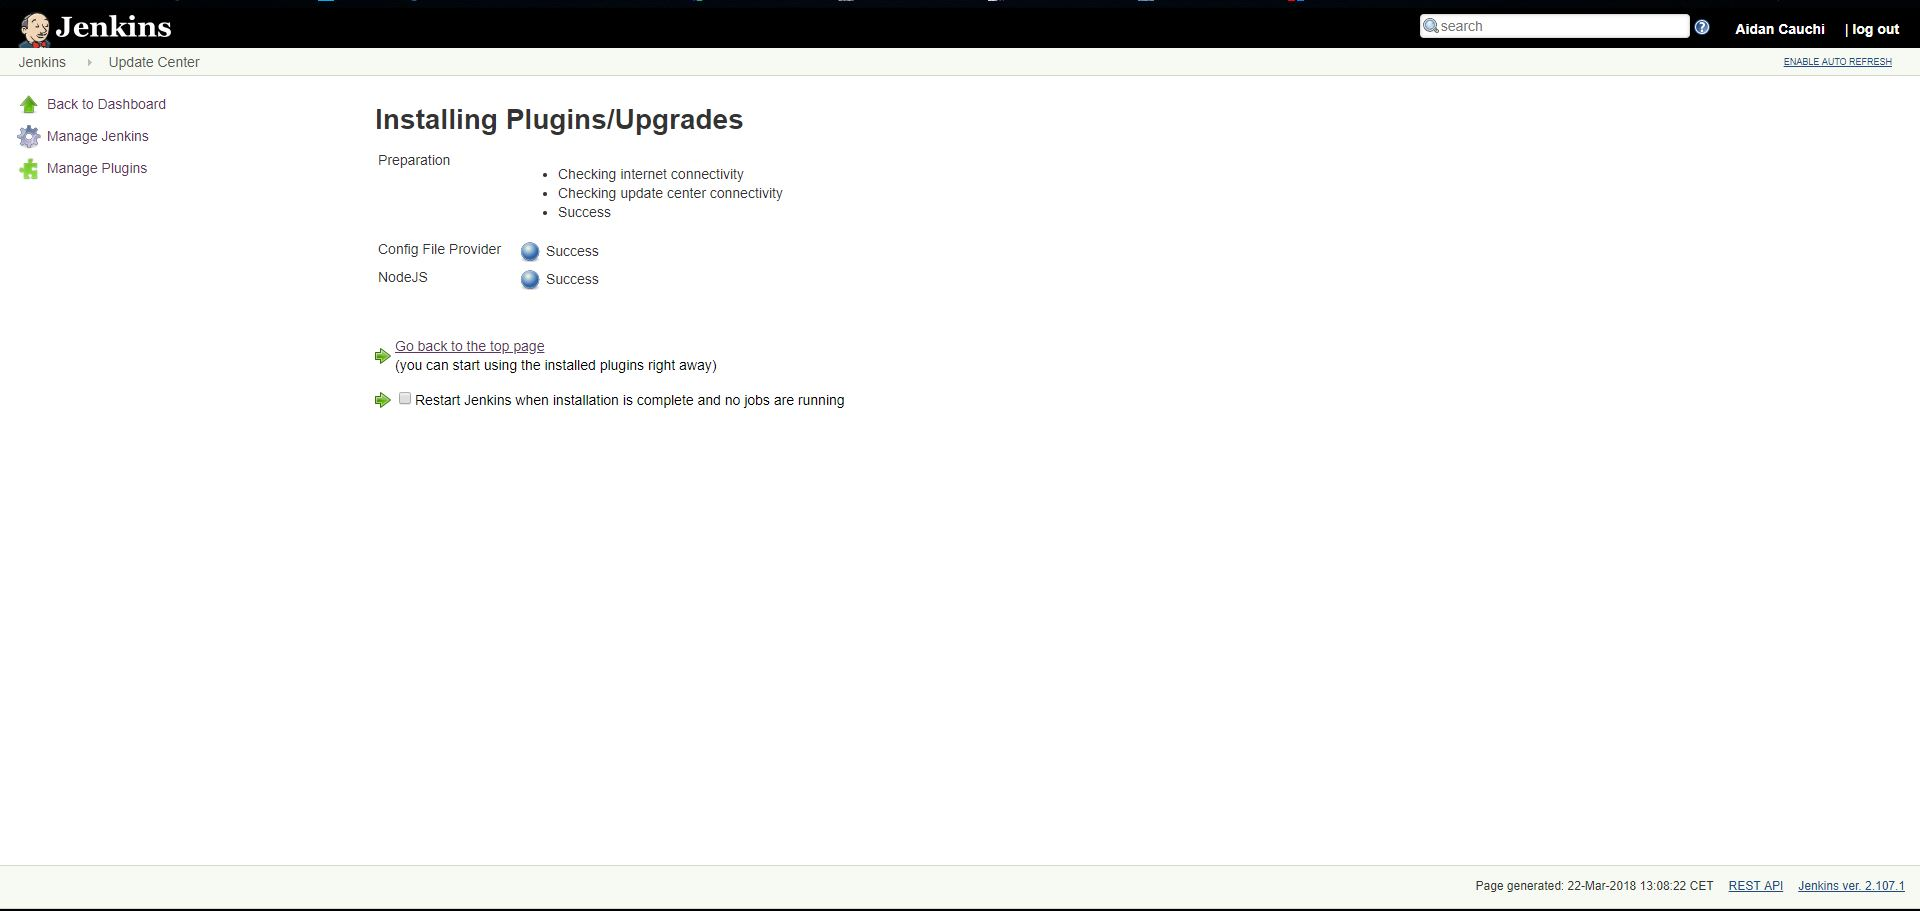
\includegraphics[width=15cm]{Jenkins/pic5.JPG}
\end{figure}
\begin{figure}[H]
  \caption{Repository and Branches}
  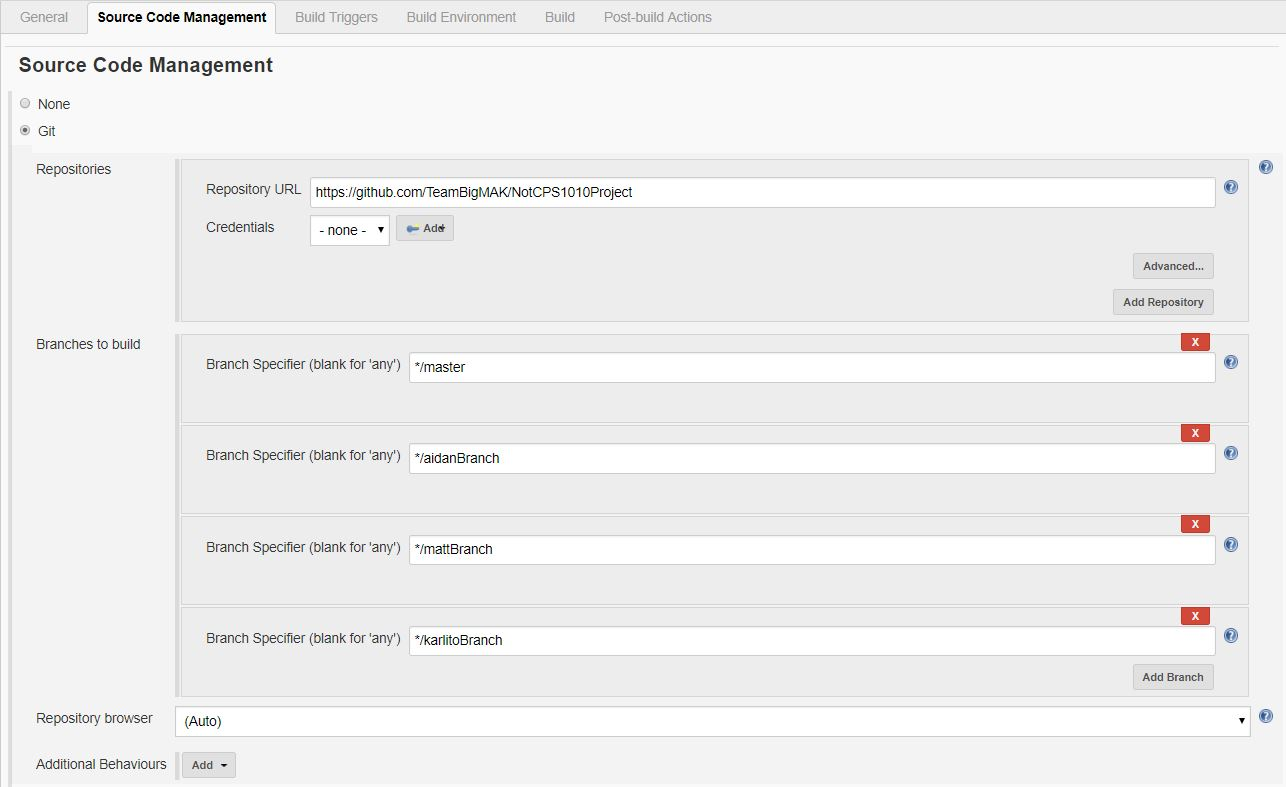
\includegraphics[width=15cm]{Jenkins/pic1.JPG}\\
  \sepspace
\end{figure}
\begin{figure}[H]
  \caption{NodeJS Build Environment}
  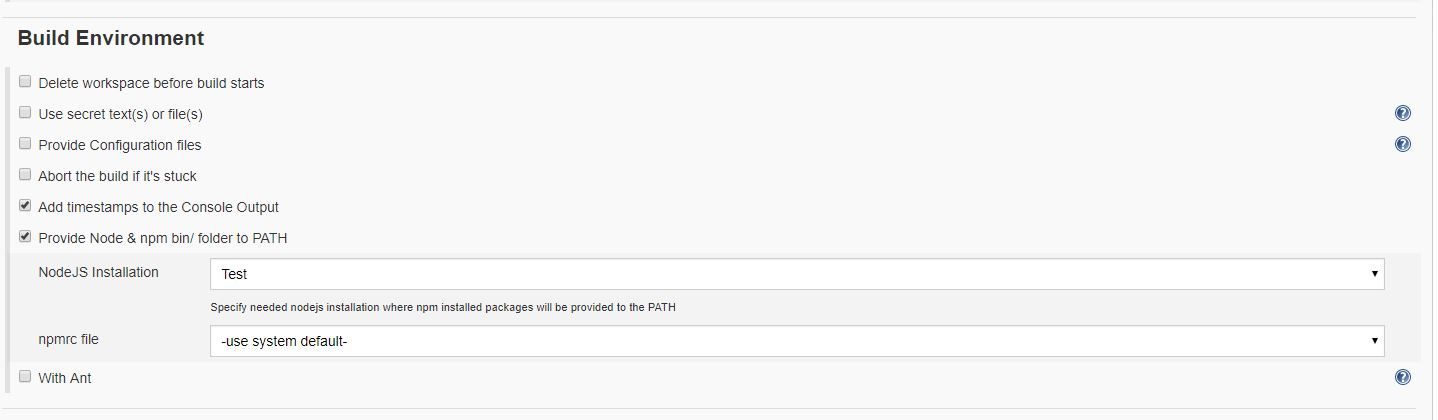
\includegraphics[width=15cm]{Jenkins/pic2.JPG}\\
  \sepspace
\end{figure}
\begin{figure}[H]
  \caption{Build Not Terminating}
  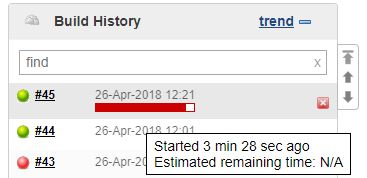
\includegraphics[width=15cm]{Jenkins/pic3.JPG}\\
  \sepspace
\end{figure}
\begin{figure}[H]
  \caption{Email Notifications}
  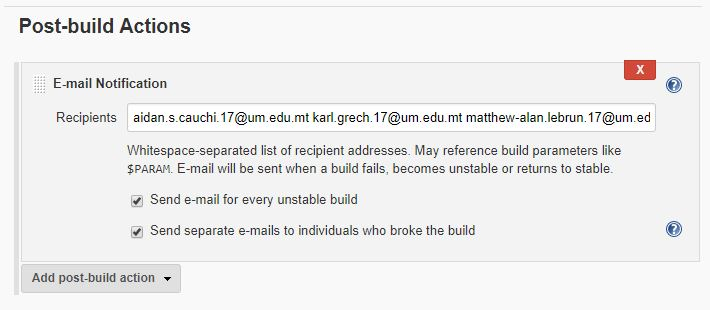
\includegraphics[width=15cm]{Jenkins/pic4.JPG}\\
  \sepspace
\end{figure}
\begin{figure}[H]
  \caption{Windows Batch Command Used to Run Node}
  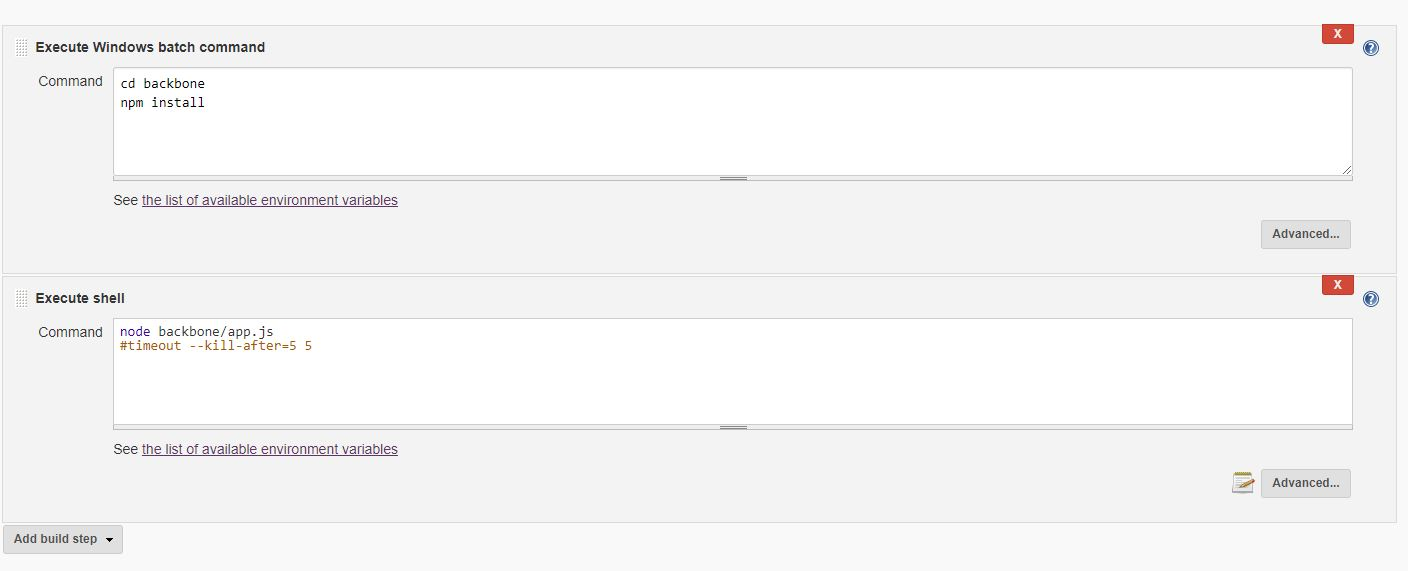
\includegraphics[width=15cm]{Jenkins/pic6.JPG}\\
  \sepspace
\end{figure}
\begin{figure}[H]
  \caption{Sample Console Output}
  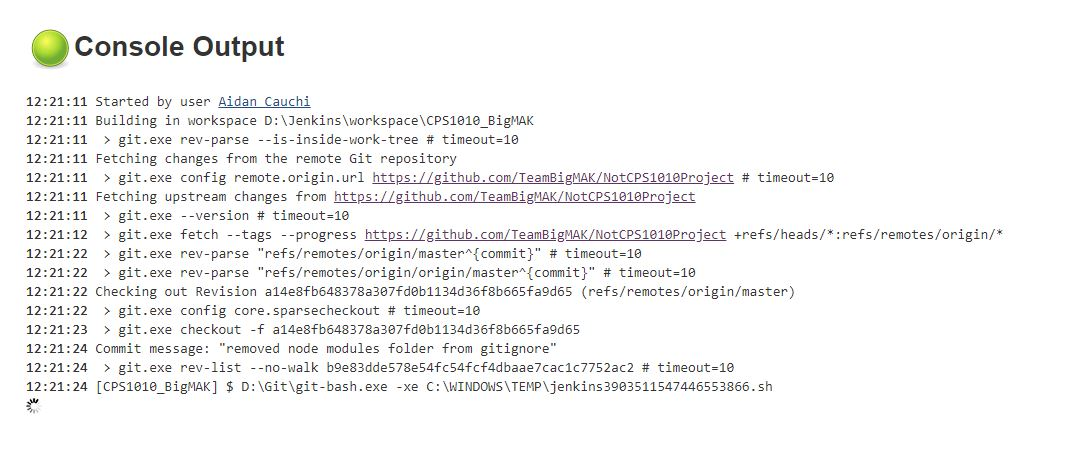
\includegraphics[width=15cm]{Jenkins/pic7.JPG}\\
  \sepspace
\end{figure}

\SectionPart{\ul{Communication Tools}}
To communicate while away from each other, the team made use of the '\textbf{Facebook
Messenger}' App for sending quick messages and planning meet ups or updating other
team members of their progress so far. For iteration plans/goals, the team made
use of an app called '\textbf{Wunderlist}', where they were able to list all the objectives
and assign them to individual team members, in an online shared list(a sort of team wall).

\begin{figure}[H]
  \caption{Wunderlist Completed and Open Tasks}
  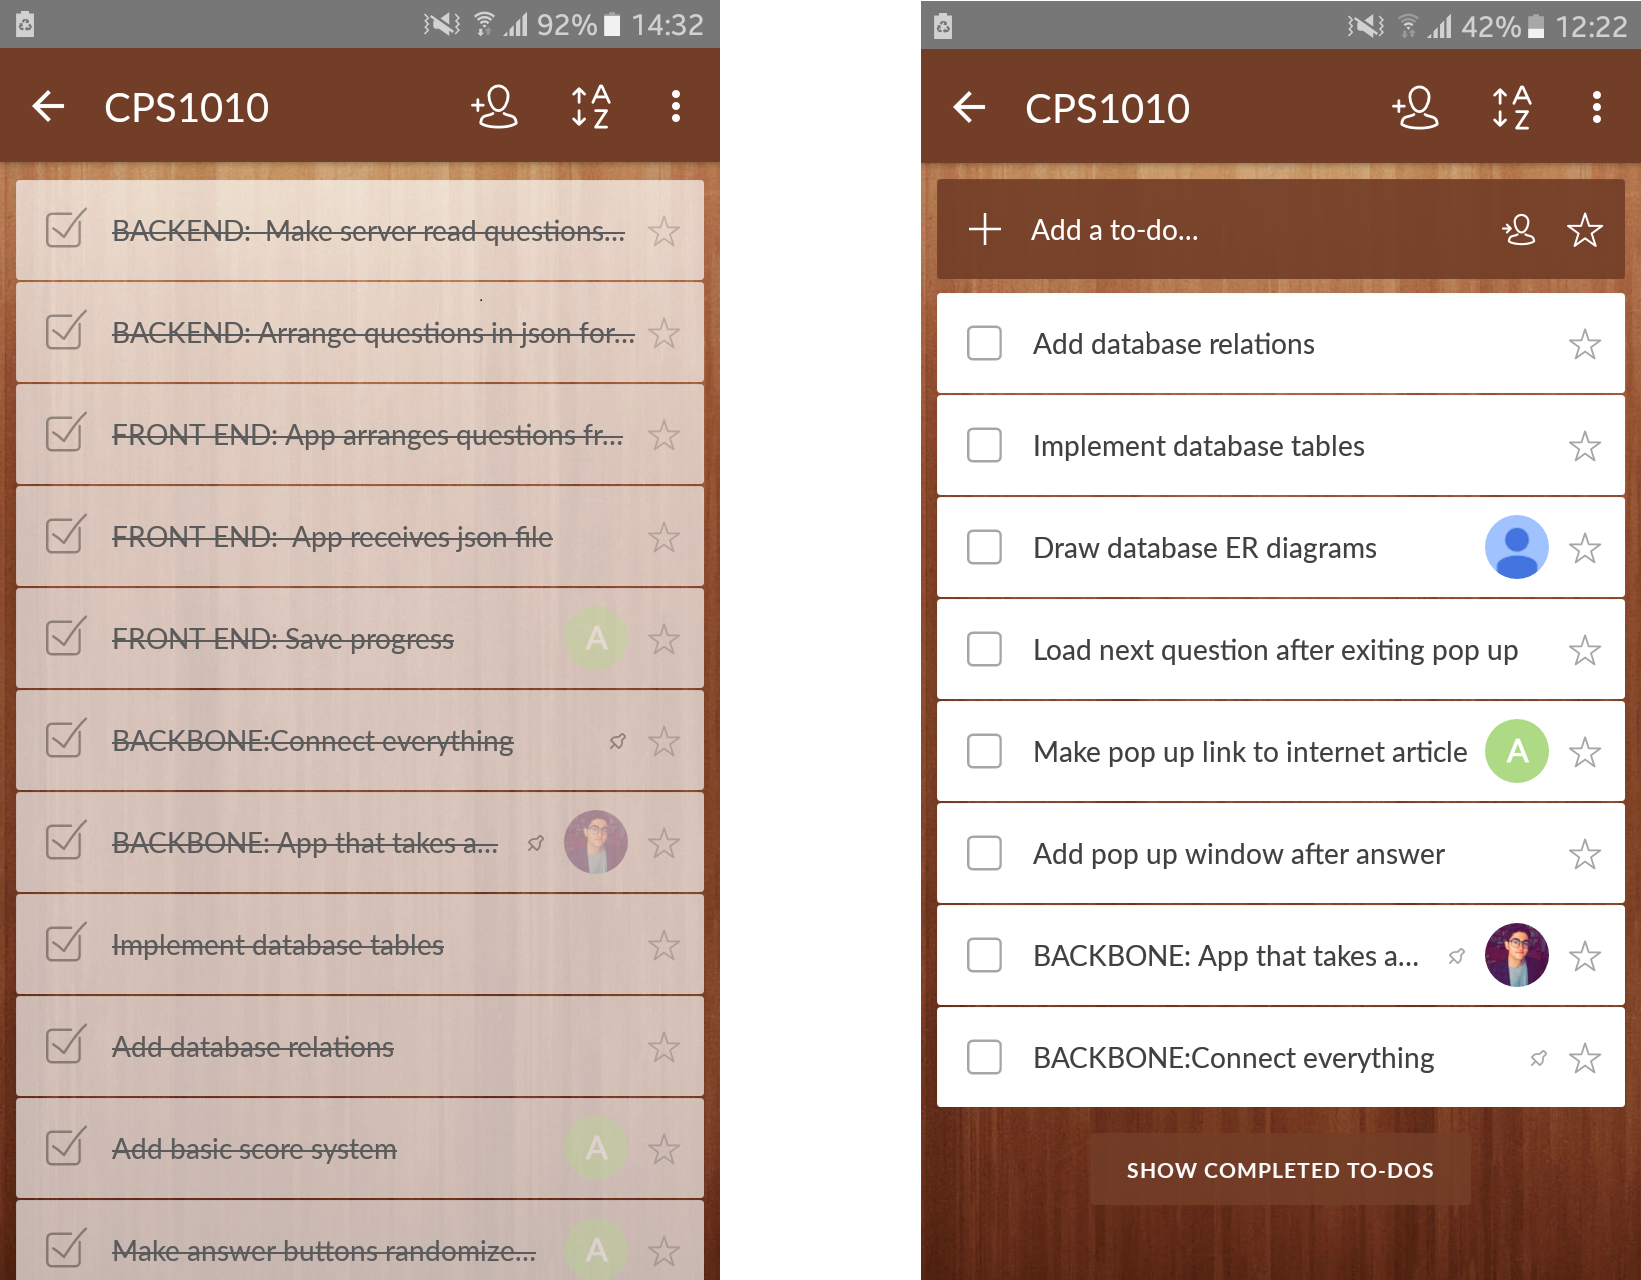
\includegraphics[width=15cm]{Wunderlist/useMe.PNG}\\
  \sepspace
\end{figure}

\sepspace

\SectionPart{\ul{Bug Tracking}}
For bug tracking the team mostly made use of the 'Wunderlist' application (mentioned
in the Communication Tools section) to take note of bugs to fix.
Occasionally, GitHub's bug tracking feature was also used for bugs that wouldn't
get fixed within iteration deadlines.

\begin{figure}[H]
  \caption{Github Issue Tracking}
  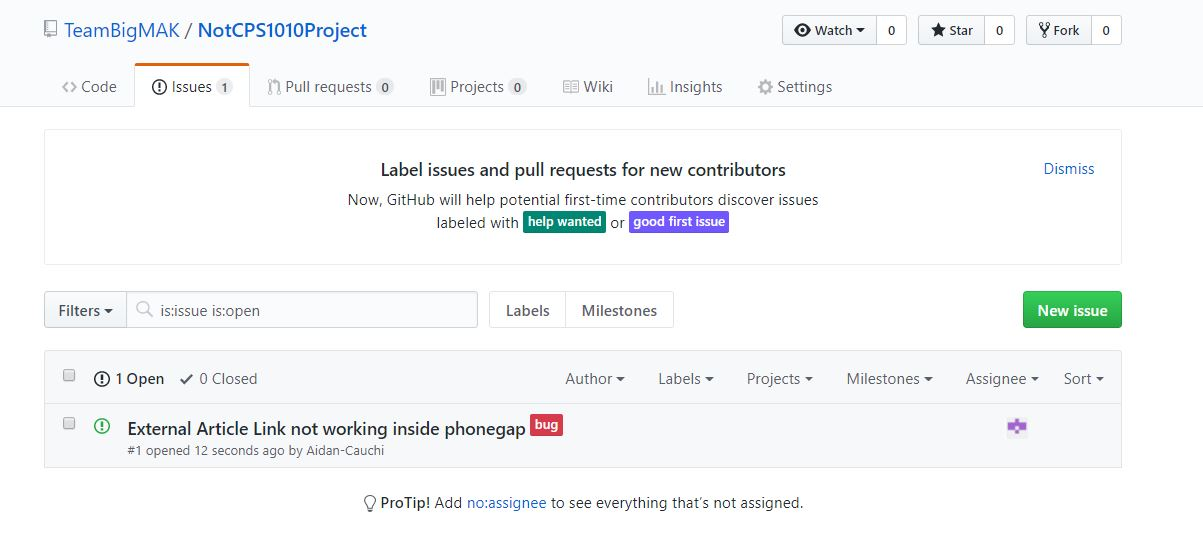
\includegraphics[width=15cm]{BugTracking/pic1.JPG}\\
  \sepspace
\end{figure}
\begin{figure}[H]
  \caption{Fixed Bug from GitHub Bug Tracker}
  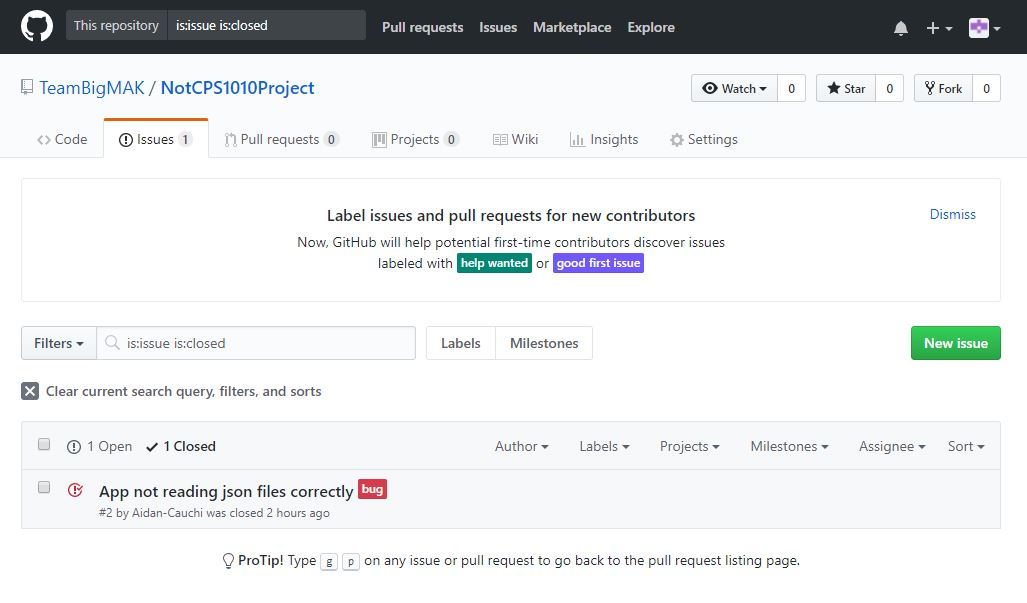
\includegraphics[width=15cm]{BugTracking/pic2.JPG}\\
\end{figure}

\sepspace

\SectionPart{\ul{Process Parameters}}
The team agreed to have iteration sprints of two weeks length. In addition, weekly group
meetings were held in the education building on University Campus every Thursday at 11:00am.
The team would discuss what was done during that week, address any pressing issues and work
concurrently for an average period of three hours.


\newpage

%%% ------------------------------------------------------------

\MainSection{Process Evolution}

\SectionPart{\ul{Iteration 0}}
\hfill \textbf{Client Meeting: 06/02/18} \\
\\
\textbf{Discussion:}\\
\noindent
In this meeting, the client expressed his desire to change the assigned idea to his own.
The idea consists of a fun politically related quiz with the aim of helping people get to
know more about politics and help to distinguish whether the "neutral/independent" sources they
are getting their information from are actually neutral after all.\\\\
\noindent
App requirements:
\begin{itemize}
	\item Cross platform availabilities for the App (being usable on Android, iOS, Windows devices)
	\item Anonymity through avoiding any sort of account making and login pages. Also, no need for the user to enter their real name and personal details but use a nickname instead.
	\item Scores for each user are sent and stored in a database. These can be then used to aid in statistical researches for example.
	\item Ability of the administrator (person in charge of the questions) to add new questions through a custom email. Questions are stored in a table in a database and questions are then updated and shown to the player.
	\item App Name and logo, however minimal importance to be given as yet.
\end{itemize}
\sepspace

\noindent
\textbf{Goals for next iteration:}\\
\noindent
Research about possible tools that can be used in the development of the app such as communication
tools and proper tools for the design and structure of the application.\\

\hfill \textbf{Internal Meeting: 08/02/18}

\begin{itemize}
	\item Agreement of the programming languages to be used - \textbf{JavaScript, NodeJS, Angular, HTML, CSS}
	\item Discussion of application to be used to convert JS to android and iOS - \textbf{PhoneGap} was found and tested
	\item Set period of research (up until the following iteration) to research and practice discussed technologies.
\end{itemize}

\hfill \textbf{Internal Meeting: 15/02/18} \\
\\
Postponed to the following week as 2 members were abroad.

\newpage
\SectionPart{\ul{Iteration 1}}
\hfill \textbf{Client Meeting: 20/02/18} \\
\\
\textbf{Discussion:}\\
\noindent
In this meeting, the client provided an in depth visual suggestion of how the system would work.
The system was to be split in two:\\\\
\noindent
\textbf{The Server Side}, which will store all questions and answers in a database and
handle all requests for questions from clients.\\\\
\noindent
\textbf{The Client Side}, including the visual representation and client functionality of the app.\\\\

\hfill \textbf{Internal Meeting: 15/02/18} \\
\\
User stories were created.\\\\
Basic Structure (backbone):
\begin{itemize}
	\item Create database (with 1 table having 1 attribute) - \textbf{20pts}
	\item Create JS based server - \textbf{63pts}
	\item Simple one page PhoneGap application - \textbf{5pts}
	\item Establish links - \textbf{20pts}
\end{itemize} \hfill total: \textbf{108pts} \\

\noindent
Front End Design:
\begin{itemize}
	\item Question Page - \textbf{20pts}
	\item Menu - \textbf{6pts}
	\item Share Results - \textbf{20pts}
	\item Colour Scheme - \textbf{5pts}
\end{itemize} \hfill total: \textbf{51pts} \\

\noindent
Back End Design:
\begin{itemize}
	\item Requests for new questions - \textbf{13pts}
	\item Store offline sessions and handle repetition - \textbf{15pts}
	\item Design of full DB - \textbf{32pts}
\end{itemize} \hfill total: \textbf{60pts} \\

\noindent
Other:
\begin{itemize}
	\item Create domain - \textbf{8pts}
	\item Adding new questions through email - \textbf{30pts}
\end{itemize} \hfill total: \textbf{38pts} \\\\

\noindent
Grand total of \textbf{257pts} - \textit{Fun fact: 257 is also the number of calories in every 100g of a BigMac}\\\\
\textbf{Sprints overview:}\\
The Project should be finished within 5 iterations, completing approximately 50pts per iteration.
\begin{itemize}
	\item Iteration 1 - Create server - \textbf{63pts}
	\item Iteration 2 - Finish backbone - \textbf{45pts}
	\item Iteration 3 - Design of full DB + Question page - \textbf{52pts}
	\item Iteration 4 - Finish back end + Finish front end - \textbf{59pts}
	\item Iteration 5 - Create domain + Addign new questions through email - \textbf{38pts}
\end{itemize}

\sepspace

\hfill \textbf{Internal Meeting: 22/02/18}

\begin{itemize}
	\item The team individually attempted to create a NodeJS app for the meeting
	\item A period of time was dedicated to bugfixing eachother's code
	\item Connected a database to a NodeJS server
	\item GitHub setup completed
	\item Wunderlist set up and tasks were assigned
\end{itemize}

\sepspace
\SectionPart{\ul{Iteration 2}}
\hfill \textbf{Client Meeting: 06/03/18} \\
\\
\textbf{Discussion:}\\
\noindent
The main focus of the meeting was discussing with the client the breakdown of
the processes required to construct the applicaton and assigning them a score based on how
difficult we thought they were and how much time we assumed they took to be done.
The client pointed out that he would prefer us to give a little more importance to the
visual representation of the app, but other than that, he agreed with our assignment of user story points.\\\\

\hfill \textbf{Internal Meeting: 08/03/18}\\
\\
\noindent
Due to the client's concern in the visual aesthetics of the application, we assigned one of the team's
members to begin working on the user interface whilst the other two continued to work on the backend.\\
\sephalfspace

\hfill \textbf{Internal Meeting: 15/03/18}\\
\\
\noindent
This meeting was dedicated solely to bugfixing backend issues the team was struggling to resolve. \\
\sepspace

\SectionPart{\ul{Iteration 3}}
\hfill \textbf{Client Meeting: 16/03/18} \\
\\
\textbf{Discussion:}\\
\noindent
\textit{Source of questions} -
The client talked to us about from where each question was being brought with the final aim
of making the app as unbiased as possible keeping in mind the final aim of educating the user
about the local politics and the political system.\\

\noindent
\textit{Type of questions} -
2 of the mentioned considerations for the quiz were the type of questions involved, and the
options to include a True or False type of question rather than only a multiple choice type of
question.\\

\noindent
\textit{JSON required} -
JSON stands for JavaScript Object Notation. The client talked about what JSON would be
required for applying a certain template to the questions, meaning that the question should
consist of the actual question, the correct answer and the wrong answers and the article link
(which links to from where the answer was brought).\\\\

\hfill \textbf{Internal Meeting: 22/03/18}\\
\\
\noindent
The team had been keeping up well with the iteration plan they created. Since this meeting was to be
the last before Easter recess, tasks were set for each member to work on and present after the recess
finished. Matthew was to work on the database design, Karl on the visuals of the question page and Aidan
was to begin adding application functionalities.\\
\sepspace

\SectionPart{\ul{Iteration 4}}
\hfill \textbf{Client Meeting: 10/04/18} \\
\\
\textbf{Discussion:}\\
\noindent
\textit{Visual overview} -
In this meeting with the Customer, we first showed him a visual progress on the application.
We added functionality we focused on was that of randomizing the answers to a question
such that the first option is not necessarily correct, but it changes every time the game is
refreshed.\\

\noindent
\textit{Releasing and Timing} -
We discussed the timing of when to release the application since releasing it in the correct
period (such as for example the budget or election period) will add a certain likeliness that the
user takes interest and makes use of the application.\\

\noindent
\textit{Further considerations} -
We discussed a bit how on a realistic level, the application is in a somewhat restricted market
since it’s a quiz and it focuses mainly on politics and political education. Thus, even for a
large percentage of teenagers (and even the population), they might see the application as
boring even though there's a lot of knowledge to gain from it. Therefore, that is why it is
imperative to add certain functionalities so as to make the application fun (and even
somewhat addicting) to use. This also depends on how well the application looks so the aim
is to make it as attractive as possible.\\

\noindent
\textit{Score System} -
The evolution of the score feature hadn't yet started. So the customer exploited this
opportunity to specify the rules for the scores. The user/player receives:
\begin{itemize}
	\item 10 points if they guess the answer on the first try
	\item 5 points if they guess the answer on the second try
\end{itemize}
This will help to create a more competitive environment such that it is not just a boring quiz
but a quiz in which you can continuously earn points.\\

\noindent
\textit{Possible game modes} -
The customer also mentioned the idea of adding different game modes within the same game
such that the user is not limited to playing just a quiz but for example a game in which you
have to match the correct title of an article to which newspaper source published it using drag
and drop.\\

\noindent
\textit{Customization} -
With regards to display, the customer focused on the fact that more importance should be
given on how the application looks on a phone rather than on desktop ie customizing it more
for small screens rather than large ones.\\

\noindent
\textit{Hosting Solution} -
A certain urge was given to finding hosting solutions such that the application, before
actually being released, would be available to show to contributors to the app and to people
who will give feedback on it.\\
\sepspace

\noindent
\textbf{Goals for next iteration:}
\begin{itemize}
	\item Work on implementing the score feature correctly
	\item Focus on adapting the app and the app layout (windows, buttons.etc) for mobile displays rather than desktop displays.
	\item Connecting the back end to the front end
	\item Search/look for server hosting solutions and present them to the customer in the next meeting
\end{itemize}
\sepspace

\hfill \textbf{Internal Meeting: 08/02/18}\\
\\
\noindent
The final internal meeting focused around polishing up the minor inconsistencies in all the
areas of the application. The team ensured that there was an established fully functional link between
the database, server and client - which could be accessed from any mobile device on the same network
as the server.\\
\sepspace

\SectionPart{\ul{Iteration 5}}
\hfill \textbf{Client Meeting: 24/04/18} \\
\\
\textbf{What was presented:}\\
\noindent
\textit{Final connection} -
The core element we had to present was the connection of the backend (mainly the database
and the items [questions, correct answers. Etc]) to the front end (the app and its features).
This was possibly the most challenging yet crucial part of the whole project as it would
ensure that the product can be released.\\

\noindent
\textit{Added functionalities} -
The load feature was successfully implemented and demonstrated in the scenario that a user
starts playing but does not complete all the available questions. In which case, if he goes back
to the start page and presses the load button, he will be taken to the next question that was to
continue from.\\
\sepspace

\noindent
\textbf{Discussion:}\\
\noindent
\textit{Added functionalities} -
Our client was very satisfied with how we managed to connect everything. He also had
suggested adding a score feature so as to make the app more competitive and addicting,
which he was also happy with.\\

\noindent
\textit{Considerations of Hosting Solutions} -
The server hosting solutions were discussed with the client. The price concern with regards to
hosting a whole/single server was raised since the prices were very expensive thus it was
agreed that the best approach would be shared hosting since they are way cheaper. We knew
hosting our application on a server that is not local and is accessible by anyone (through a
valid URL) was something our client wanted to see he wanted to show the application to
other people who might be able to give feedback both on how the app looks and with regards
to how it works so we saw that as a bit of a dull moment.\\

\noindent
\textit{UI Considerations} -
Some more refinements were to be made to the UI, mainly with regards to the overlay; ie the
window that appears to tell the user whether the option they chose is correct or wrong. It also
then includes a ‘Learn More’ button which links to the document or webpage from where the
information from the question was taken.\\
\noindent
The client inquired as to whether the responses/clicks of the user were being sent to a
database or in general if any data used for statistical purposes was being saved however the
answer was in the negative as our main goal was to load the permanently/hard-coded saved
data from the database and eventually show it to the end user.\\

\noindent
\textit{Suggestions on start-up} -
After some personal testing of the features done by the client himself, he stated that according
to him, the user shouldn’t have the play button each time he starts the app especially since
pressing on this button would reset your scores and data. However the play button would
appear only for the first time the page is loaded and then no more [unless the app is
uninstalled and reinstalled or all its data is erased for example]. It also seemed that the client
did not want any sort of menu whenever the app is loaded (not for the first time) but changed
his mind and saw it better that the user; once he enters the app, is immediately shown the next
question on the screen; (provided there are any new questions [which were added] in the
database).\\

\noindent
\textit{Final Verdict} -
On a more positive general note, the client was very impressed with how the team's work was
carried out overall and also the way in which the work was organised and split (into iterations
etc) and stated considerations of working together on this application in the coming Summer.
This encouraged the team as it was taken as a sign that the customer was happy since a lot of
his needs for the application were being met.\\\\

\newpage

%%% ------------------------------------------------------------

\MainSection{Testing}

\SectionPart{\ul{Ad-hoc Testing}}
\textit{What is it?}\\
An informal testing approach done without any reference to any plan or test
cases usually with the aim of breaking the system and detecting which defects
lead to this. One of the key elements in this type of testing is improvisation;where the
testers do what deems necessary to find any bugs in the code. An in-depth knowledge of the
system is a crucial requirement.\\
\sephalfspace

\noindent
\textit{How was it used?}\\
Ad-hoc testing was used in various stages of the app development, particularly since our
time was somewhat limited, since we had to follow the plans of action per each iteration,
so especially at the final parts of each iteration, to check that the feature or build was almost
bug-free (since no software is ever error free). At later stages of the development, since the UI had
started to connect with the back-end,we exploited the UI and tried to find bugs by interacting with
it and finding possible routes (that a user could potentially do) that could lead to errors.\\
\sepspace

\SectionPart{\ul{Bottom-up Testing}}
\textit{What is it?}\\
Bottom-up testing is one of the many possible approaches to integration testing. Rather than
create the main module and then move on to sub module; bottom up inverts the approach and the developers
first work on the (smaller) sub-modules, and each time adding up the latter modules to go up one level to a
module that incorporates these sub-modules. If you visualize it, it is sort of a pyramid where the main/final
module is the point on the top and as you go further down, you will find the stuff that sustains/makes up the
core thing. In bottom up we start from the bottom of the pyramid and keep building on it till we reach the top.\\
\sephalfspace

\noindent
\textit{How was it used?}\\
In our case,with the idea of the pyramid in mind, the top part;the main module was basically the final app idea.
To give some practical examples,creating the database tables (with all the questions and other information) was
a vital step in the whole process, and although this was a big step, it still was considered a sub-module since
it helped in creating the final thing. Managing to get the data from the database was another thing and finally
combining the getting of the data with the ui was another step upward in the pyramid to reach the final aim.
Some of the sub-modules actually weren't in the initial pyramid plan but as the work evolved, we realized that
the particular sub-module shouldn't be overlooked. On a smaller scale,the score functionality was a small
module within itself but it was important to complete/add to the UI, which along with the backend and the
connection between them would combine to form the final app.\\
\sepspace

\SectionPart{\ul{Integration Testing}}
\textit{What is it?}\\
Integration testing is concerned with testing how different modules interact in cohesion, rather than with
the individual modules themselves. It is used to identify situations such as data being lost between modules,
one module creating a fault in another module and creating a major undesirable side-effect when combining modules.\\
\sephalfspace

\noindent
\textit{How was it used?}\\
This was a very vital type of testing especially at a later stages when the database was successfully
created and the front-end along with all the javascripts scripts were done. The testing was done to
ensure that the connection between the client with the server and the server with database were successfully
working. This could be checked by simply running the application and seeing whether the questions load from
the database and whether upon selection of a possible answer to a question, the overlay/window indicating
whether the chosen answer is correct or incorrect is displayed. Also,this type of testing is recommended when
different modules are written by different programmers so indirectly, it was necessary to do so.\\

\sepspace
%%% ------------------------------------------------------------

\MainSection{Customer Feedback}
The following pages contain the customer feedback form review.

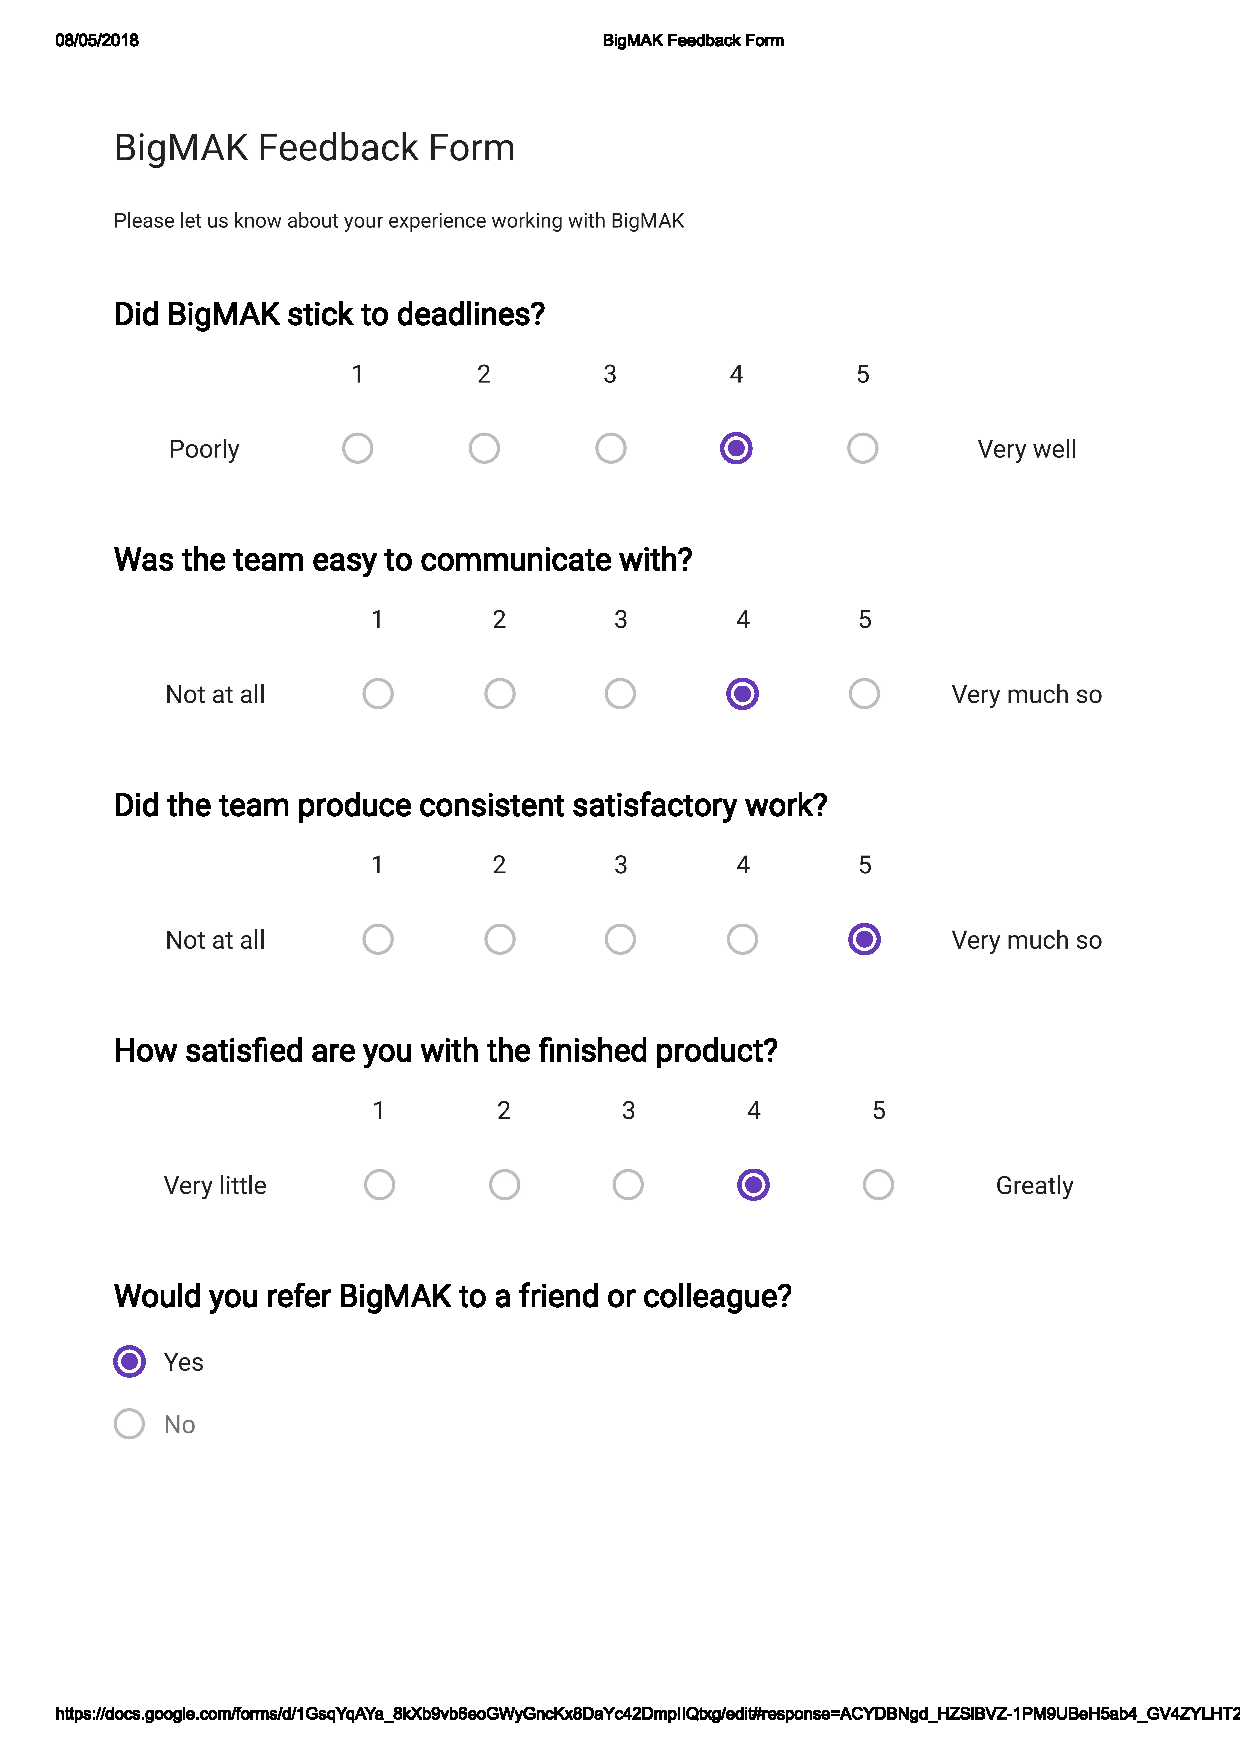
\includepdf[pages=-,pagecommand={},width=\textwidth]{feedback.pdf}


\newpage

%%% ------------------------------------------------------------

\MainSection{Program Walkthrough}
To facilitate testing, the team decided that it would be best to work with a
web based application(for compatibility).\\

\noindent
Upon connecting to the PhoneGap server (which was used for testing) the user is
greeted with the menu screen. Furthermore, when the user connects to the server/website,
a signal is sent to the backend server to retrieve the questions from the database
and send them back to the phone, where they are organized for the play session.
Moreover, in the menu screen, the user may choose to select one of three
buttons: Play, Options and Load. The options button currently lacks any functionality
as it was placed there for UI testing.\\

\noindent
Pressing the play button causes the app to start loading the questions and to reset previously saved data.
Each question has a question number, the question itself, 3 wrong answers and 1 correct answer.
Should the user press the correct answer during the first try, they are immediately
congratulated, given 10 points and are given the option to either continue playing
or learn more about the topic of the question. Otherwise, they are expected to try
again for one last time but are rewarded 5 points if they get it right during the
second try. If the user fails to answer the questions within both tries, the application
displays the correct answer and loads the next question. It is important to know
that the app saves user progress after every question the user answers.\\

\noindent
If the user presses the load button instead, they would continue playing from the question
number they previously stopped at.

%%% ------------------------------------------------------------


\end{document}
